\documentclass[usenames,dvipsnames,aspectratio=169,12pt]{beamer}
\usepackage{tikz}
\usetikzlibrary{tikzmark,positioning,intersections}
\usepackage[customcolors]{hf-tikz}
\usepackage{microtype}
\usepackage{amsmath,amssymb,mathpartir,stmaryrd}
\usepackage[style=alphabetic,backref=true,maxbibnames=1000,natbib=true]{biblatex}
\usepackage{wasysym}
\usepackage{textcomp}
\usepackage[normalem]{ulem}
\usepackage{listings}
\usepackage{color}
\usepackage{xparse}
\usepackage{newtxmath}
\usepackage[nameinlink,capitalize,noabbrev]{cleveref}

\definecolor{JadeGreen}{RGB}{0,168,107}
\definecolor{MunsellPurple}{RGB}{159,0,197}
\definecolor{LightGrey}{gray}{0.9}
\definecolor{CobaltBlue}{RGB}{0,71,171}
\definecolor{FireBrick}{RGB}{228,34,23}
\definecolor{Alabaster}{RGB}{250,250,250}

\hypersetup{colorlinks,urlcolor=CobaltBlue}

\usetheme[numbering=counter]{metropolis}
\setbeamertemplate{navigation symbols}{}
\setbeamertemplate{itemize items}{$\bullet$}

\NewDocumentCommand{\Arr}{m m}{#1 \to #2}
\NewDocumentCommand{\Fun}{m m}{\mathsf{fun}\, #1 \Rightarrow #2}
\NewDocumentCommand{\App}{m m}{#1(#2)}
\NewDocumentCommand{\Nat}{}{\mathsf{Nat}}
\NewDocumentCommand{\Zero}{}{\mathsf{zero}}
\NewDocumentCommand{\Succ}{m}{\mathsf{succ}(#1)}
\NewDocumentCommand{\Vect}{m m}{\mathtt{Vec}(#1, #2)}
\NewDocumentCommand{\Nil}{}{\mathsf{nil}}
\NewDocumentCommand{\Cons}{m m}{#1 {:} #2}
\NewDocumentCommand{\Lang}{m}{\mathtt{#1}}

\NewDocumentCommand{\Nf}{m m}{\llbracket #1 : #2 \rrbracket}

\title{Implementing Type Theory}
\author{\textbf{Daniel Gratzer}\inst{1} \and Jonathan Sterling\inst{2} \and Lars Birkedal\inst{1}}
\institute{\inst{1} This University \smiley{} \\ \inst{2} Not This University \frownie{}}
\date{May 24, 2019}

\begin{document}
\begin{frame}[noframenumbering]
  \titlepage
\end{frame}

\begin{frame}
  \frametitle{Some Terminology}
  Languages classify expressions into different \emph{types}
  (\texttt{\textcolor{CobaltBlue}{int}},
  \texttt{\textcolor{CobaltBlue}{string}},
  \texttt{\textcolor{CobaltBlue}{char}}).

  \begin{description}
  \item[Type System] The rules for what expressions belong to which types.
  \item[Type-Checker] The program that makes sure we follow the rules.
  \end{description}

\end{frame}

\begin{frame}
  \frametitle{Setting the Scene}

  What is type theory? Type theory is a....
  \begin{itemize}
  \setbeamercolor{itemize item}{fg=CobaltBlue}
  \item programming language with a rich type system.
  \setbeamercolor{itemize item}{fg=red}
  \item framework for reasoning about mathematical objects.

  \end{itemize}
  \pause
  \centering
  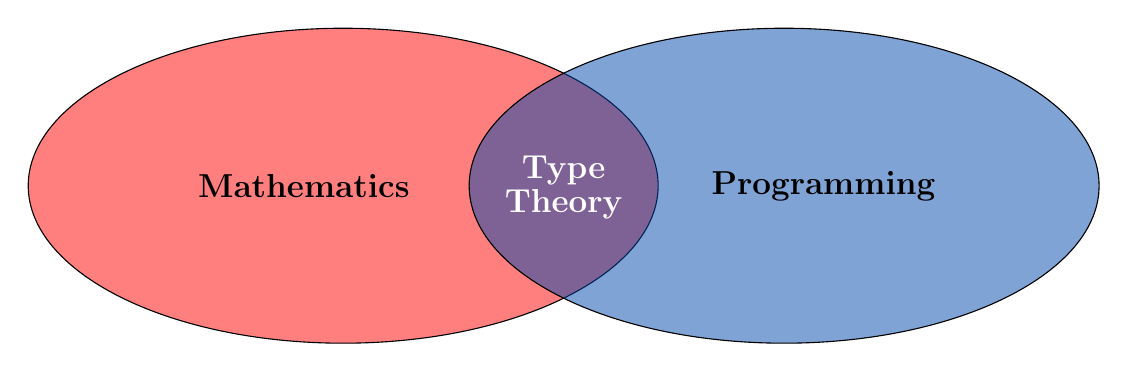
\begin{tikzpicture}
    \begin{scope}[shift={(3cm,-4.3cm)}, fill opacity=0.5,
      mytext/.style={text opacity=1,font=\large\bfseries}]

      \draw[fill=red, draw = black] (-2.8,0) ellipse (4 and 2);
      \draw[fill=CobaltBlue, draw = black,name path=circle 2] (2.8,0) ellipse (4 and 2);

      \node[mytext] at (-3.3,0) (B) {Mathematics};
      \node[mytext] at (3.3,0) (C) {Programming};
      \node[mytext] at (0,0) (C) {{\color{White} $\overset{\text{\large Type}}{\text{Theory}}$}};
    \end{scope}
  \end{tikzpicture}
\end{frame}


\begin{frame}
  \frametitle{A Concrete Issue}
  Set aside the questions of \textcolor{Red}{mathematics} and \textcolor{Blue}{programming} for a
  second.
  \bigskip

  Type theory has functions
  \setbeamercolor{block body example}{bg=LightGrey}
  \begin{example}
    \[
      \App{\Lang{useful\_\tikzmark{fun}function}}{\Lang{important\_\tikzmark{arg}argument}}
    \]
  \end{example}
  \onslide<1>{When is this application well-typed?}
  
\begin{tikzpicture}[
    remember picture,
    overlay,
    expl/.style={draw=Alabaster,fill=orange!30,rounded corners,text width=3cm},
    arrow/.style={Gray!70!black,ultra thick,->,>=latex}
    ]
    \node<2->[expl]
    (funex)
    at (-5,-0.75cm)
    {must have type $\Arr{A}{B}$};
    \node<3->[expl]
    (argex)
    at (4.5,-0.75cm)
    {must have type $C$};
    \node<4->
    at (0, -0.75cm)
    {\textbf{We must also have $A = C$}};
    \draw<2->[arrow]
    (funex) to ([xshift=-0.5ex,yshift=-0.5ex]{pic cs:fun});
    \draw<3->[arrow]
    (argex) to ([xshift=-0.5ex,yshift=-0.5ex]{pic cs:arg});
  \end{tikzpicture}
\end{frame}

\begin{frame}
  \frametitle{How Hard is Type-Checking?}
  What should we take away from this example?
  \begin{enumerate}
  \item In order to type-check, we must check if two types are equal.
  \item We need a program checking type equality.
  \end{enumerate}
\end{frame}

\begin{frame}
  \frametitle{Just Type Equality?}
  Deciding type equality is always a problem but we have fancier types:
  \begin{align*}
    \Vect{\Lang{A}}{\Lang{n}} &&
    \text{A list of $\Lang{A}$s of length $\Lang{n}$}
  \end{align*}
  \pause
  We need more than type equality... we need term equality too!
  \[
    \Vect{\Lang{A}}{2 * \Lang{n}} \stackrel{?}{=} \Vect{\Lang{A}}{\Lang{n} + \Lang{n}}
  \]
\end{frame}

\begin{frame}
  \frametitle{The Mess We're In}
  In order to implement type theory we must check the equality of terms.
  \begin{enumerate}
  \item So this is completely impossible in a Turing-complete language\footnote{Python, Java, C,
      C++, PostScript, and Magic the Gathering are all Turing-complete}.
  \item Actually it's impossible in many Turing-\emph{incomplete} languages as well.
  \item Many equalities we expect are impossible to automatically check:
    \[
      f = g \iff \text{for all } x,\ \App{f}{x} = \App{g}{x}
    \]
  \end{enumerate}
\end{frame}

\begin{frame}
  \frametitle{Modern Type Theory}
  The central balancing act is then defining an equality relation which is
  \begin{itemize}
  \item strong enough to match our \textcolor{Red}{mathematical} intuitions.
  \item simple enough that we can \textcolor{Blue}{implement} it.
  \end{itemize}
\end{frame}

\begin{frame}
  \frametitle{Implementing Type Theory}
  Once this is done we can write programs with very strong guarantees:
  \begin{alignat*}{2}
    &\Lang{map} : (\Lang{A} \to \Lang{B}) &&\to \Vect{\Lang{A}}{\Lang{n}} \to \Vect{\Lang{B}}{\Lang{n}}\\
    &\App{\Lang{map}}{\Lang{f}, []} &&\triangleq []\\
    &\App{\Lang{map}}{\Lang{f}, \Lang{h} :: \Lang{t}} &&\triangleq \App{\Lang{f}}{\Lang{h}} :: \App{\Lang{map}}{\Lang{f}, \Lang{t}}
  \end{alignat*}
  See our ICFP'19 paper: \url{https://jozefg.github.io/modal.pdf}
\end{frame}

\begin{frame}
  \frametitle{Conclusions (Some of the Stuff I Skipped)}
  I cut out a lot of cool stuff in this talk:
  \begin{itemize}
  \item Using type theory, we can ``run'' math proofs.
  \item We can use computer science to explore mathematics.
  \item We can use maths to inspire better PLs.
  \end{itemize}
  Many unexplored and interesting questions remain...
\end{frame}

\begin{frame}
  \frametitle{The LogSem Group}
  If this sounds interesting, please come talk to us!
  \begin{figure}
    \begin{tabular}{ccccc}
    {\includegraphics[height = 0.5in]{aslan.jpg}}      &
    {\includegraphics[height = 0.5in]{lars.jpg}}       &
    {\includegraphics[height = 0.5in]{bas.jpg}}        &
    {\includegraphics[height = 0.5in]{jaco.jpg}}       &
    {\includegraphics[height = 0.5in]{danil.jpg}}     \\
    {\includegraphics[height = 0.5in]{sabine.jpg}}     &
    {\includegraphics[height = 0.5in]{alix.png}}       &
    {\includegraphics[height = 0.5in]{kristoffer.jpg}} &
    {\includegraphics[height = 0.5in]{johan.jpg}}      &
    {\includegraphics[height = 0.5in]{martin.jpg}}    \\
    {\includegraphics[height = 0.5in]{jeppe.png}}      &
    {\includegraphics[height = 0.5in]{aina.jpg}}       &
    {\includegraphics[height = 0.5in]{jakob.png}}      &
    {\includegraphics[height = 0.5in]{marit.png}}      &
    {\includegraphics[height = 0.5in]{mathias.jpg}}   \\
    {\includegraphics[height = 0.5in]{simon.jpg}}      &
    {\includegraphics[height = 0.5in]{lau.jpg}}        &
    {\includegraphics[height = 0.5in]{soeren.jpg}}     &
    {\includegraphics[height = 0.5in]{me.jpg}}         &
    {\includegraphics[height = 0.5in]{andreas.jpg}}
    \end{tabular}
  \end{figure}
\end{frame}

\end{document}
